\documentclass[11pt]{article}

% XeTeX engine (tectonic): do NOT load inputenc; UTF-8 is native.
\usepackage[margin=1in]{geometry}
\usepackage{amsmath,amssymb}
\usepackage{booktabs}
\usepackage{array}
\usepackage{graphicx}
\usepackage{xcolor}
\usepackage{tikz}
\usetikzlibrary{arrows.meta,positioning,fit,backgrounds}
\usepackage{pgfplots}
\pgfplotsset{compat=1.18}
\usepackage[numbers,sort&compress]{natbib}
\usepackage[colorlinks=true,linkcolor=black,citecolor=blue,urlcolor=blue]{hyperref}
\usepackage{titlesec}

\titleformat{\section}{\normalfont\large\bfseries}{\thesection}{0.6em}{}
\titleformat{\subsection}{\normalfont\normalsize\bfseries}{\thesubsection}{0.5em}{}
\setlength{\parskip}{0.35em}
\setlength{\parindent}{0pt}

\newcommand{\layer}[1]{\textsc{#1}}
% left-ragged fixed-width column: avoids underfull \hbox in narrow cited cells
\newcolumntype{L}[1]{>{\raggedright\arraybackslash}p{#1}}

% Title kept text-only (no \textbf / \\) so it extracts cleanly into
% plain-text metadata (digest/email/HTML); vertical spacing is handled by the
% \vspace before \maketitle below.
\title{Defense in Depth for Language-Model Applications:
A Practitioner's Taxonomy of Evaluation, Retrieval Quality, Guardrails,
and Hallucination Mitigation}

\author{Yash Singh\\
\small IIIT Una}

\date{18 July 2026}

\begin{document}
\vspace*{-2em}
\maketitle

\begin{abstract}
Large language models (LLMs) fail in production for reasons that no single
technique fully addresses: they fabricate facts, drift from retrieved evidence,
ignore instructions, and answer confidently when they should abstain. The
research literature offers a large and fast-moving catalogue of remedies, but
practitioners face these methods as a disconnected toolbox rather than a
coherent engineering discipline. This paper is a practitioner-oriented synthesis
that organizes reliability techniques for LLM applications into four composable
layers: (i) \emph{evaluation}, the measurement substrate that turns
reliability from a vibe into a number; (ii) \emph{retrieval quality}, which
governs whether a model is even given the evidence it needs; (iii)
\emph{inference-time reliability}, self-checking and abstention that catch
errors before they leave the model; and (iv) \emph{guardrails}, the
programmable input/output controls that bound behavior. We map common failure
modes to the layers that mitigate them, contrast the dominant methods on cost,
latency, and the failures they actually catch, and propose a reference
architecture that composes the layers as defense in depth. Our contribution is
synthesis and framing rather than new empirical results: we argue that
reliability is achieved not by any one method but by stacking cheap, imperfect
filters, where distinct filters extend coverage across failure classes and
redundant, independent filters drive the residual of any single class down
multiplicatively. We close with the open
problems that this framing exposes, chiefly evaluator trust, calibrated
abstention, and the absence of end-to-end reliability budgets.
\end{abstract}

\section{Introduction}

A demo that works once and a product that works reliably are separated by a wide
gap that LLMs make unusually treacherous. A retrieval-augmented assistant can
answer a hundred questions correctly and then, on the hundred-and-first,
confidently cite a policy that does not exist. The failure is not a crash with a
stack trace; it is fluent, plausible, and invisible until a user is harmed. This
is the central engineering problem of applied LLM work: the failure surface is
open-ended and the failures are silent.

The research community has responded with a rich catalogue of methods:
retrieval augmentation to ground generation in evidence
\citep{lewis2020rag,shuster2021retrieval}, self-consistency and verification to
reduce reasoning errors \citep{wang2023selfconsistency,dhuliawala2023cove},
black-box hallucination detectors \citep{manakul2023selfcheckgpt},
fine-grained factuality metrics \citep{min2023factscore}, automated evaluation
frameworks \citep{es2023ragas,saadfalcon2024ares,zheng2023mtbench}, and
programmable guardrails \citep{rebedea2023nemo,bai2022constitutional}. Each is
valuable, but each is typically presented in isolation, benchmarked against a
narrow slice of failures. A practitioner who has read all of these papers still
lacks the thing they most need: a way to reason about \emph{how the pieces fit
together} into a system whose overall failure rate is acceptable.

This paper offers that framing. We make three claims.

\textbf{(1) Reliability is a stack, not a technique.} No single method drives
production failure rates low enough. Grounding reduces but does not eliminate
hallucination; self-checking catches some but not all fabrications; guardrails
block known-bad patterns but not novel ones. The path to reliability is defense
in depth: multiple cheap, imperfect filters arranged so that residual error
decays roughly multiplicatively rather than additively.

\textbf{(2) The layers are mostly separable, and each answers a distinct
question.} We organize the toolbox into four layers, summarized in
Figure~\ref{fig:arch}: evaluation (\emph{how wrong are we?}), retrieval quality
(\emph{did the model get the evidence?}), inference-time reliability
(\emph{does the model's own output survive scrutiny?}), and guardrails
(\emph{is the output within allowed bounds?}). Failure modes map to layers
(Table~\ref{tab:failures}), which lets a team locate the cheapest layer that
addresses a given class of failure. The separation is a modeling convenience,
not a hard boundary: adaptive methods like Self-RAG \citep{asai2024selfrag}
deliberately fuse retrieval and self-critique into one loop, and we name such
exceptions where they arise. The blur is benign because the taxonomy's job is to
route a failure to the \emph{cheapest} layer that catches it, not to forbid a
method from spanning two.

\textbf{(3) Evaluation is the load-bearing layer.} Every other layer is only as
trustworthy as the measurement that validates it. Because human labels do not
scale, teams increasingly rely on LLM-as-judge and reference-free metrics
\citep{zheng2023mtbench,es2023ragas}, which import their own reliability
problem. We treat evaluator trust as the discipline's central open question.

Our aim is a map, not a new algorithm, and we are explicit about what is new
and what is borrowed. The genuine unit of novelty is the \emph{cross-family
composition}: existing surveys catalogue methods \emph{within} a single failure
family, hallucination \citep{ji2023hallucination,huang2023hallucination} or
retrieval \citep{gao2023ragsurvey}, whereas we treat the whole pipeline as the
object of analysis and ask how methods from different families compose into one
system with a single, budgetable failure rate. The taxonomy, the failure-to-layer
mapping, and the reference architecture are the scaffolding for that argument
rather than novel artifacts in themselves; ``defense in depth'' is a borrowed
security metaphor that we make quantitative through the residual-error and budget
models of Section~\ref{sec:arch}. The payoff is practical: a working engineer can
use the composition to decide what to build first and where the residual risk
lives.

\section{Related Work}
\label{sec:related}

Our closest neighbors are surveys, and the distinction is deliberate. The
hallucination surveys of \citet{ji2023hallucination} and
\citet{huang2023hallucination}, and the RAG survey of \citet{gao2023ragsurvey},
are exhaustive \emph{within} their family but stop at the family boundary: they
taxonomize causes and list mitigations without asking how a retrieval fix and a
guardrail trade off against each other under one shared error budget. Evaluation
surveys and frameworks \citep{liang2023helm,es2023ragas,saadfalcon2024ares}
similarly treat measurement as an end in itself rather than as the instrument
that tunes every other layer. What none of these provide, and what we contribute,
is the \emph{cross-family} view: a single request path in which methods from
different families are composed, and a residual-error model
(Section~\ref{sec:arch}) that makes their interaction budgetable.

The individual mechanisms we cite are, of course, prior work: retrieval
grounding \citep{lewis2020rag}, self-checking and verification
\citep{wang2023selfconsistency,dhuliawala2023cove,manakul2023selfcheckgpt},
uncertainty and abstention
\citep{kadavath2022know,kuhn2023semantic,angelopoulos2021conformal}, programmable
and learned guardrails
\citep{rebedea2023nemo,inan2023llamaguard,bai2022constitutional}, and attribution
\citep{gao2023citations}. Our claim is not to improve any of them but to supply
the missing arithmetic of how they stack.

\section{A Taxonomy of Failure}
\label{sec:failures}

Reliability is undefined until failure is. We adopt a coarse but operationally
useful taxonomy, aligned with the hallucination surveys of
\citet{ji2023hallucination} and \citet{huang2023hallucination} but extended to
the application concerns that dominate production.

\textbf{Intrinsic hallucination.} The output contradicts the provided source or
context. In a RAG system this is a \emph{faithfulness} failure: the retrieved
passage says one thing, the answer says another. It is the most tractable
failure because the ground truth (the context) is present at inference time.

\textbf{Extrinsic hallucination.} The output asserts facts that cannot be
verified against any provided source and happen to be false. Closed-book
factual errors live here. These are harder because verification requires
knowledge the system does not hold.

\textbf{Retrieval failure.} The correct evidence was never surfaced: wrong
chunk, poor recall, stale index, or a query the retriever could not match. No
downstream layer can fix an answer built on absent evidence.

\textbf{Instruction and format violation.} The output ignores a constraint:
wrong schema, disallowed content, exceeded length, broken tool call. These are,
in many deployments, among the highest-frequency production failures and,
fortunately, the easiest to detect deterministically.

\textbf{Safety and policy violation.} The output is harmful, discloses private
data, or is successfully jailbroken \citep{perez2022redteaming,ganguli2022redteaming}.

\textbf{Miscalibration.} The output is wrong \emph{and} confident, or the system
answers when it should have abstained. Calibration cuts across the other
categories and determines whether the system knows what it does not know
\citep{kadavath2022know}.

Table~\ref{tab:failures} maps each failure to the layers that most cheaply
mitigate it. The recurring lesson is that failures are caught most cheaply
close to their source: retrieval failures at the retrieval layer, format
violations at the guardrail layer, and only the residue by expensive
inference-time self-checking.

\begin{table*}[t]
\centering
\small
\renewcommand{\arraystretch}{1.25}
\begin{tabular}{@{}L{3.1cm} L{4.3cm} L{4.8cm} L{2.6cm}@{}}
\toprule
\textbf{Failure mode} & \textbf{Where it originates} & \textbf{Cheapest mitigating layer} & \textbf{Detectable?} \\
\midrule
Intrinsic hallucination & Generator drifts from context & Inference-time faithfulness check; RAG eval \citep{es2023ragas} & Yes (context present) \\
Extrinsic hallucination & Parametric knowledge is wrong & Retrieval grounding \citep{lewis2020rag}; self-check \citep{manakul2023selfcheckgpt} & Partially \\
Retrieval failure & Retriever recall / index & Retrieval quality layer; Self-RAG \citep{asai2024selfrag} & Yes (offline eval) \\
Instruction / format & Decoding ignores constraint & Output guardrail (schema/validator) & Yes (deterministic) \\
Safety / policy & Adversarial or unlucky input & Input+output guardrails \citep{rebedea2023nemo}; RLAIF \citep{bai2022constitutional} & Partially \\
Miscalibration & No abstention signal & Confidence + abstention \citep{kadavath2022know} & Hard \\
\bottomrule
\end{tabular}
\caption{Failure modes mapped to the layer that most cheaply mitigates them.
``Detectable?'' asks whether the failure can be caught automatically at
acceptable cost, which determines whether it can be gated in a pipeline.}
\label{tab:failures}
\end{table*}

\section{Layer 1: Evaluation}
\label{sec:eval}

Evaluation is placed first not because it runs first at inference time but
because it is the precondition for every other layer: a mitigation you cannot
measure is a mitigation you cannot trust or tune.

\textbf{Static benchmarks} such as HELM \citep{liang2023helm} and TruthfulQA
\citep{lin2022truthfulqa} give comparable, reproducible scores across models but
answer a different question than production teams ask. They measure a model in
the abstract; they do not measure \emph{your} application on \emph{your}
distribution. They are necessary for model selection and nearly useless for
regression-testing a specific pipeline.

\textbf{Behavioral and unit-style testing}, in the spirit of CheckList
\citep{ribeiro2020checklist}, closes part of that gap by asserting invariants
(paraphrase invariance, directional expectations, known-answer probes) on the
actual system. This is the LLM analogue of the unit test and belongs in CI.

\textbf{Reference-free and LLM-as-judge evaluation} has become the practical
default because gold labels do not scale. MT-Bench and Chatbot Arena
\citep{zheng2023mtbench} popularized using a strong model as grader;
RAGAS \citep{es2023ragas} and ARES \citep{saadfalcon2024ares} specialize this
for retrieval systems, decomposing quality into faithfulness (is the answer
grounded in retrieved context?), answer relevance, and context relevance.
FActScore \citep{min2023factscore} pushes toward fine-grained factual precision
by decomposing a generation into atomic facts and verifying each.

The catch is that an LLM judge is itself an LLM subject to every failure in
Section~\ref{sec:failures}: it has position and verbosity biases, it can be
gamed, and it inherits the blind spots of its training. The practitioner's
mitigation is to treat the judge as a measurement instrument that must itself be
calibrated against a small human-labeled set, to prefer decomposed rubric
scoring over holistic 1--10 ratings, and to track judge--human agreement as a
first-class metric. Evaluation does not remove the reliability problem; it
relocates it to a place where it can be sampled cheaply.

\begin{table*}[t]
\centering
\small
\renewcommand{\arraystretch}{1.25}
\begin{tabular}{@{}L{3.0cm} L{3.4cm} L{4.0cm} L{4.2cm}@{}}
\toprule
\textbf{Approach} & \textbf{Measures} & \textbf{Strength} & \textbf{Limitation} \\
\midrule
Static benchmark \citep{liang2023helm,lin2022truthfulqa} & Model, in the abstract & Comparable, reproducible & Not your distribution \\
Behavioral tests \citep{ribeiro2020checklist} & Invariants on your system & Deterministic, CI-friendly & Only what you thought to assert \\
LLM-as-judge \citep{zheng2023mtbench} & Subjective quality at scale & Cheap, flexible & Judge bias; needs calibration \\
RAG-specific \citep{es2023ragas,saadfalcon2024ares} & Faithfulness, relevance & Decomposed, actionable & Depends on judge quality \\
Atomic factuality \citep{min2023factscore} & Per-fact precision & Fine-grained & Costly; needs a knowledge source \\
\bottomrule
\end{tabular}
\caption{Evaluation approaches. No single row is sufficient; teams combine
static benchmarks for model selection, behavioral tests in CI, and
reference-free judges for continuous monitoring.}
\label{tab:eval}
\end{table*}

\section{Layer 2: Retrieval Quality}
\label{sec:retrieval}

Retrieval augmentation is the highest-leverage reliability intervention because
it attacks extrinsic hallucination at the root: a model that is handed the
answer is far less likely to invent one \citep{lewis2020rag,shuster2021retrieval,gao2023ragsurvey}.
But RAG relocates rather than removes the problem. It introduces a new failure
mode, retrieval failure, and a new dependency, the faithfulness of the generator
to what it retrieved.

Three sub-problems dominate in practice. \emph{Recall}: did the relevant chunk
enter the candidate set at all? This is governed by chunking strategy, embedding
quality, and hybrid (lexical plus dense) retrieval, and it is bounded above by
the index. No re-ranker recovers a document that was never indexed.
\emph{Precision and ordering}: is the relevant chunk near the top, given finite
context budget? Re-ranking addresses this. \emph{Grounding}: given good context,
does the generator actually use it? This is measured by faithfulness metrics
\citep{es2023ragas} and is where intrinsic hallucination hides.

Adaptive schemes such as Self-RAG \citep{asai2024selfrag} let the model decide
\emph{when} to retrieve and \emph{whether} retrieved passages are relevant,
emitting reflection tokens that critique its own use of evidence. This begins to
blur Layer~2 into Layer~3: retrieval quality and self-critique become a single
loop. The practitioner's takeaway is that retrieval must be evaluated as its own
component, with its own metrics (recall@\emph{k}, context relevance) measured
independently of end-to-end answer quality, because a good final answer can mask
a broken retriever that the model happened to route around, and a bad answer can
hide a perfect retriever undone by a generator that ignored it.

\section{Layer 3: Inference-Time Reliability}
\label{sec:inference}

The third layer operates on the model's own output at generation time, without
external knowledge, exploiting a useful asymmetry: verifying a claim is often
easier than producing it, and sampling the model multiple times exposes its
uncertainty.

\textbf{Self-consistency} \citep{wang2023selfconsistency} samples several
reasoning paths and takes the majority answer, trading compute for accuracy on
tasks with a checkable final answer. \textbf{Chain-of-Verification}
\citep{dhuliawala2023cove} has the model draft an answer, generate verification
questions, answer them independently, and revise, which measurably cuts
fabrication in list and entity tasks. \textbf{SelfCheckGPT}
\citep{manakul2023selfcheckgpt} exploits the observation that fabricated content
is unstable across samples: if independently sampled responses disagree on a
fact, that fact is likely hallucinated, giving a black-box detector that needs
no external database.

Cutting across these is \textbf{calibration and abstention}. Models carry usable
signal about their own correctness \citep{kadavath2022know}; the reliability
question is whether the system converts that signal into a decision to abstain,
defer to a human, or hedge. Two threads sharpen the raw signal. \emph{Semantic
entropy} \citep{kuhn2023semantic} measures uncertainty at the level of meaning
rather than tokens, clustering sampled generations by semantic equivalence so
that a model that says the same thing five different ways is correctly scored as
confident, while one that contradicts itself is flagged; this makes the
SelfCheckGPT intuition quantitative. \emph{Conformal prediction}
\citep{angelopoulos2021conformal} goes further, wrapping any black-box scorer in a
distribution-free procedure that returns prediction sets (or an abstention) with a
finite-sample coverage guarantee, turning an ad hoc threshold into one with a
provable error rate. In many production settings a calibrated ``I don't know'' is
worth more than a marginally more accurate guess, because it converts a silent
failure into a visible, routable one.

The cost of this layer is real: self-consistency and verification multiply token
usage and latency. This makes Layer~3 the natural place for a \emph{selective}
policy, spending extra compute only on inputs the cheaper layers flag as
uncertain or high-stakes.

\section{Layer 4: Guardrails}
\label{sec:guardrails}

Guardrails are the deterministic and semi-deterministic controls that bound what
enters and leaves the model. They are conceptually the outermost shell in
Figure~\ref{fig:arch} because they need no understanding of correctness, only of
\emph{allowed shape}.

\textbf{Output validation} is the cheapest and most reliable guardrail:
schema/JSON validation, regex and type checks, tool-argument validation, and
retry-on-invalid. Because format violations are deterministically detectable
(Table~\ref{tab:failures}), this layer can drive that failure class to near
zero, and no probabilistic method should be used where a validator suffices.

\textbf{Programmable rails} such as NeMo Guardrails \citep{rebedea2023nemo}
generalize this to semantic policies: topical boundaries, canonical-form
dialogue flows, and fact-checking rails, expressed in a controlled language that
sits outside the model. \textbf{Learned classifier rails}, exemplified by Llama
Guard \citep{inan2023llamaguard}, complement rule-based policies with a
purpose-trained model that classifies both prompts and responses against an
explicit safety taxonomy, catching the semantic violations a regex cannot express
while remaining a separate, auditable component rather than a property of the
generator. \textbf{Input rails} handle jailbreak and injection detection before
the model is invoked, informed by red-teaming that systematically discovers
failure inputs \citep{perez2022redteaming,ganguli2022redteaming}.

\textbf{Attribution rails} sit between guardrails and evaluation: requiring the
model to emit inline citations to its retrieved sources, and rejecting or
regenerating any claim whose citation does not support it, converts an unverifiable
assertion into a checkable one \citep{gao2023citations}. Attribution is a
particularly cheap output rail in a RAG system because the evidence is already in
context, and it directly attacks the intrinsic-hallucination class of
Section~\ref{sec:failures}.

\textbf{Value alignment via feedback}, exemplified by Constitutional AI
\citep{bai2022constitutional}, is a guardrail baked into the weights rather than
bolted on around them: the model is trained to critique and revise its own
outputs against an explicit set of principles. This complements rather than
replaces external rails, since a trained-in disposition is cheaper at inference
but harder to audit, update, and prove than an external rule.

The design principle for this layer is that guardrails should be composed by
\emph{cost and determinism}: run the cheapest deterministic check first, and
reserve model-based rails for what deterministic checks cannot express.

\section{A Reference Architecture}
\label{sec:arch}

Figure~\ref{fig:arch} composes the four layers into a single request path. The
arrangement encodes the paper's thesis: filters are ordered so that each removes
the failures it catches most cheaply, and only the residue reaches the next,
more expensive filter. The layer \emph{numbers} follow exposition order rather
than request order: the guardrail layer (Section~\ref{sec:guardrails}) appears at
\emph{both} ends of the path, as input rails at the top and output rails at the
bottom, because the same deterministic machinery bounds both the request and the
response.

\begin{figure}[t]
\centering
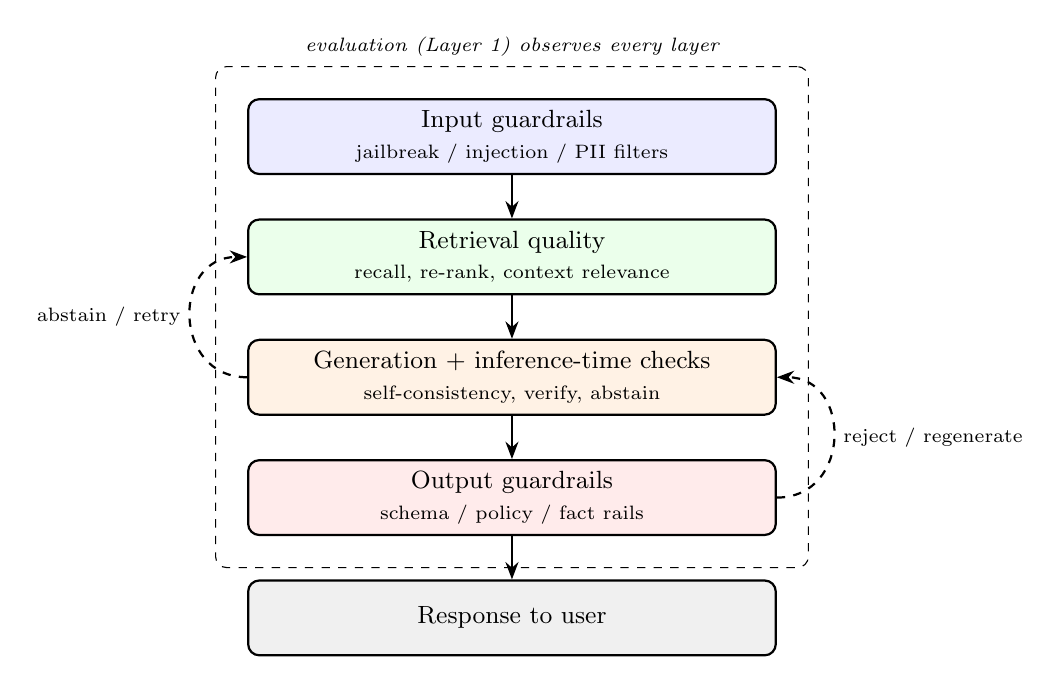
\begin{tikzpicture}[
  node distance=0.55cm,
  every node/.style={font=\small},
  layerbox/.style={draw, rounded corners, minimum width=6.7cm,
    minimum height=0.95cm, align=center, thick},
  flow/.style={-{Stealth[length=2.2mm]}, thick},
]
\node[layerbox, fill=blue!8]  (input)  {Input guardrails \\ \scriptsize jailbreak / injection / PII filters};
\node[layerbox, fill=green!8, below=of input] (retr)
  {Retrieval quality \\ \scriptsize recall, re-rank, context relevance};
\node[layerbox, fill=orange!10, below=of retr] (gen)
  {Generation + inference-time checks \\ \scriptsize self-consistency, verify, abstain};
\node[layerbox, fill=red!8, below=of gen] (out)
  {Output guardrails \\ \scriptsize schema / policy / fact rails};
\node[layerbox, fill=gray!12, below=of out] (user)
  {Response to user};

\draw[flow] (input) -- (retr);
\draw[flow] (retr) -- (gen);
\draw[flow] (gen) -- (out);
\draw[flow] (out) -- (user);

% feedback / abstention edges (both routed left to avoid the frame label)
\draw[flow, dashed] (gen.west) to[out=180,in=180, looseness=1.6]
      node[left, font=\scriptsize] {abstain / retry} (retr.west);
\draw[flow, dashed] (out.east) to[out=0,in=0, looseness=1.6]
      node[right, font=\scriptsize] {reject / regenerate} (gen.east);

\begin{scope}[on background layer]
\node[draw, dashed, rounded corners, fit=(input)(retr)(gen)(out),
      inner sep=0.4cm,
      label={[font=\scriptsize\itshape]above:evaluation (Layer 1) observes every layer}] {};
\end{scope}
\end{tikzpicture}
\caption{Defense-in-depth reference architecture. Solid arrows are the request
path; dashed arrows are corrective loops (abstention, regeneration). Evaluation
(Layer~1, dashed frame) is not on the request path but instruments every layer,
producing the metrics that tune the others.}
\label{fig:arch}
\end{figure}

Two properties of this composition matter more than any single box.

\textbf{Two mechanisms, not one.} It is tempting to summarize defense in depth as
``errors decay multiplicatively,'' but that slogan conflates two distinct effects,
and only one of them is actually multiplicative. \emph{Coverage} is a union
effect: distinct layers catch distinct failure classes, so adding a layer that
handles a previously unhandled class simply removes that class from the residual.
Coverage is what the failure-to-layer map (Table~\ref{tab:failures}) buys, and it
is additive in the classes it eliminates, not multiplicative. \emph{Redundancy}
is the multiplicative effect, and it applies only \emph{within} a class: if $m$
independent filters each miss a fraction $\epsilon_1,\dots,\epsilon_m$ of the
\emph{same} failure instances, the fraction surviving all of them is
$\prod_{i}\epsilon_i$. Consider one high-stakes class guarded by three redundant,
mechanistically different filters, each missing a fraction $\epsilon = 0.3$ of
instances (these figures are pedagogical, not measured). Their residual is
$0.3^3 = 0.027$, which beats a single stronger filter at $\epsilon = 0.1$, but it
costs roughly three inferences instead of one, the tradeoff the budget objective
below makes explicit. Crucially, this compounding buys nothing for a class that
only one of the three filters can even see: redundancy shrinks a term, it does not
create coverage. Figure~\ref{fig:residual} plots this decay and contrasts it with
the additive coverage effect.

Writing $C$ for the set of failure classes, $p_c$ for the base rate of class $c$,
and $L(c)$ for the layers redundantly covering it, the overall residual is a sum
over classes of a per-class product,
\[
  R \;\approx\; \sum_{c \in C} p_c \, \rho_c \!\!\prod_{i \in L(c)} \epsilon_{i,c},
  \qquad \rho_c \ge 1 .
\]
Coverage decides which terms are nonzero; redundancy shrinks each surviving term.
The factor $\rho_c$ is where the linchpin assumption is made honest: $\rho_c = 1$
is the idealized independent case (the clean product), and $\rho_c > 1$ measures
how much correlated failures inflate the residual when a hard input defeats
several of class $c$'s filters at once. Because $\rho_c$ is a property of the
inputs and the filters jointly, it must be \emph{measured}, not assumed to be $1$;
carrying it explicitly is the standing argument for making redundant layers
\emph{mechanistically different} (a deterministic validator and an LLM judge fail
on different inputs, pushing $\rho_c$ toward $1$).

\begin{figure}[t]
\centering
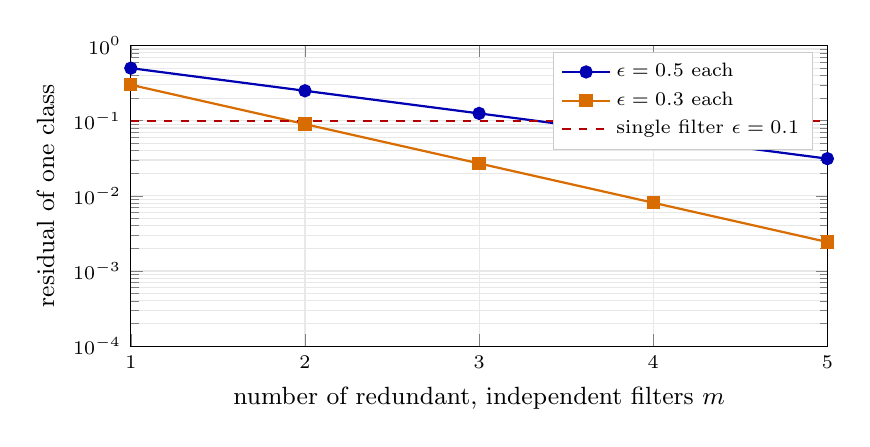
\begin{tikzpicture}
\begin{axis}[
  width=0.86\linewidth, height=5.4cm,
  xlabel={number of redundant, independent filters $m$},
  ylabel={residual of one class},
  ymode=log, log basis y=10,
  xmin=1, xmax=5, ymin=1e-4, ymax=1,
  xtick={1,2,3,4,5}, grid=both, grid style={gray!18},
  legend cell align=left,
  legend style={font=\scriptsize, at={(0.98,0.98)}, anchor=north east, draw=gray!40},
  tick label style={font=\scriptsize}, label style={font=\small},
]
\addplot[thick, mark=*, blue!70!black]   coordinates {(1,0.5)(2,0.25)(3,0.125)(4,0.0625)(5,0.03125)};
\addplot[thick, mark=square*, orange!85!black] coordinates {(1,0.3)(2,0.09)(3,0.027)(4,0.0081)(5,0.00243)};
\addplot[thick, dashed, red!70!black] coordinates {(1,0.1)(5,0.1)};
\legend{$\epsilon=0.5$ each, $\epsilon=0.3$ each, single filter $\epsilon=0.1$}
\end{axis}
\end{tikzpicture}
\caption{Redundancy within a single failure class is multiplicative: $m$
independent filters of per-filter miss rate $\epsilon$ leave residual
$\epsilon^{m}$ (log scale). Three $\epsilon=0.3$ filters (orange) reach $0.027$,
below a single $\epsilon=0.1$ filter (dashed), at the cost of running three
filters. This decay applies only \emph{within} a class the filters share; adding a
filter for a \emph{new} class instead removes that class's term from $R$ additively
(coverage). Rates are illustrative, not measured.}
\label{fig:residual}
\end{figure}

\textbf{Cost is spent where risk is.} The cheap deterministic layers (input and
output guardrails) run on every request; the expensive layers (multi-sample
inference-time checks) run selectively, gated by a confidence or stakes signal.
A system that runs Chain-of-Verification on every request has misallocated its
compute; one that runs it only on flagged requests approaches the same
reliability at a fraction of the cost.

This reframes reliability engineering as \emph{budget allocation}. Weighting each
class in $R$ by the harm $h_c$ of a failure in it, the goal is to choose the
filter placement $L(\cdot)$ that minimizes expected residual harm subject to a
per-request cost ceiling,
\[
  \min_{L(\cdot)} \ \sum_{c \in C} p_c\, h_c\, \rho_c \!\!\prod_{i \in L(c)} \epsilon_{i,c}
  \quad \text{s.t.} \quad \sum_{i} \mathbb{1}[i \text{ runs}]\,\mathrm{cost}(i) \le B,
\]
where $\mathrm{cost}(i)$ is filter $i$'s latency-plus-token price and $\rho_c \ge 1$
is the same correlation factor as in $R$, kept inside the objective on purpose: an
allocation optimized under the independence assumption $\rho_c = 1$ can be badly
wrong precisely on the correlated, hard inputs that matter most, so the term must
travel with the objective rather than be relegated to a caveat. Selective
execution enters as the observation that a filter need not run on every request:
gating an expensive filter on a cheap uncertainty signal lowers its amortized
cost without changing its $\epsilon$ on the inputs that matter. We do not solve
this program. We observe that the field optimizes individual $\epsilon_{i,c}$ (a
better retriever, a better judge) without ever writing down the objective they
feed into, nor collecting the $p_c$, $\epsilon_{i,c}$, $h_c$, and $\rho_c$ needed
to estimate it. That objective, and its data, is, to our knowledge, still largely
absent from both the research literature and production practice.

\textbf{A worked micro-instantiation.} To show the objective is runnable rather
than merely aspirational, consider a toy pipeline with three failure classes and
two candidate filters (all numbers illustrative). Class rates and per-failure harm
are: format violation ($p=0.10$, $h=1$), intrinsic hallucination ($p=0.05$,
$h=5$), and jailbreak ($p=0.02$, $h=20$). Filter $A$ is a cheap deterministic
validator ($\mathrm{cost}=1$) that catches format violations well
($\epsilon=0.05$) but is blind to the other two ($\epsilon=1$). Filter $B$ is an
LLM judge ($\mathrm{cost}=4$) that partially catches hallucination and jailbreak
($\epsilon=0.3$ on each) but not format. Under a per-request budget $B=5$ we can
afford both, and assuming near-independence ($\rho_c \approx 1$) the expected
residual harm is
\[
  \underbrace{0.10\cdot1\cdot0.05}_{\text{format}}
  +\underbrace{0.05\cdot5\cdot0.3}_{\text{halluc.}}
  +\underbrace{0.02\cdot20\cdot0.3}_{\text{jailbreak}}
  = 0.005 + 0.075 + 0.120 = 0.20 .
\]
Had the same budget instead bought two copies of the judge $B$ (dropping the
validator), format violations would run unguarded ($0.10\cdot1\cdot1 = 0.10$)
while the doubled judge drives the other two down by $0.3^2$, for a total of
$0.10 + 0.0225 + 0.036 = 0.16$ \emph{only if} the two judge passes fail
independently; at a realistic $\rho \approx 3$ for two copies of the \emph{same}
model that becomes $0.10 + 0.0675 + 0.108 = 0.28$, worse than the mixed
allocation. The lesson the arithmetic makes concrete: mechanistically diverse
filters beat redundant identical ones once $\rho$ is honest, and the cheapest
deterministic layer is almost never the one to drop.

\section{Discussion, Limitations, and Open Problems}
\label{sec:discussion}

\textbf{Limitations, stated plainly.} This is a synthesis and position paper, and
we are careful not to claim more. The two load-bearing quantitative objects, the
residual model $R$ and the budget program of Section~\ref{sec:arch}, are
\emph{illustrated} with pedagogical constants, not \emph{validated} on a measured
pipeline; we present no case study estimating real $p_c$, $\epsilon_{i,c}$, $h_c$,
or the correlation factors $\rho_c$. The contribution is therefore a framework and
a vocabulary for reasoning about composition, not evidence that the framework
predicts a specific system's failure rate. We believe the honest framing is
exactly this, a practitioner's map that the field can now instrument, and the
single most valuable next step is one end-to-end case study on a real RAG or
agentic pipeline that measures the quantities the model assumes, especially the
cross-layer correlation $\rho_c$ it currently only names.

The layered framing also clarifies what is solved and what is not.

\textbf{Evaluator trust is the bottleneck.} Every layer is tuned against a
metric, and the metrics increasingly come from LLM judges
\citep{zheng2023mtbench,es2023ragas}. We lack a rigorous, cheap way to bound how
much to trust an automated evaluator on a novel distribution. Until we do,
reported reliability gains rest on a foundation that is itself unvalidated.

\textbf{Calibrated abstention is underdeveloped.} Models carry self-knowledge
signal \citep{kadavath2022know}, but converting it into a well-calibrated,
task-appropriate policy that abstains or defers to a human at the right moment
remains ad hoc.

\textbf{Agentic pipelines invert the arithmetic.} Every mechanism in this paper
is single-turn, yet the multiplicative composition that \emph{helps} within a
redundantly covered class turns hostile the moment a system chains steps, as it
does in agents that interleave reasoning and acting over a trajectory
\citep{yao2023react}. If an agent takes $n$ dependent actions and each succeeds
independently with probability $1-\delta$, end-to-end success is $(1-\delta)^n$
and decays geometrically (Figure~\ref{fig:agentic}): a per-step error rate of
$\delta = 0.05$, unremarkable in isolation, yields only a $0.60$ success rate over
a ten-step trajectory. The link back to the framework is direct: the per-step
failure rate $\delta$ is precisely the single-turn residual of
Section~\ref{sec:arch}, $\delta = R = \sum_c p_c\, \rho_c \prod_{i \in L(c)}
\epsilon_{i,c}$, evaluated at one step. Every layer multiplies its $\epsilon$ into
$\delta$ and so sets the \emph{base} of the exponential, but no single-turn layer
can touch the \emph{exponent} $n$. Controlling $n$ (shorter plans, checkpointing,
recovery) and decorrelating consecutive steps therefore become first-order
reliability levers that the single-turn literature surveyed here barely addresses.
Extending the failure-to-layer map and the budget objective of
Section~\ref{sec:arch} to whole trajectories, where the base rates $p_c$
themselves compound with depth, is the most consequential direction this framing
leaves open.

\begin{figure}[t]
\centering
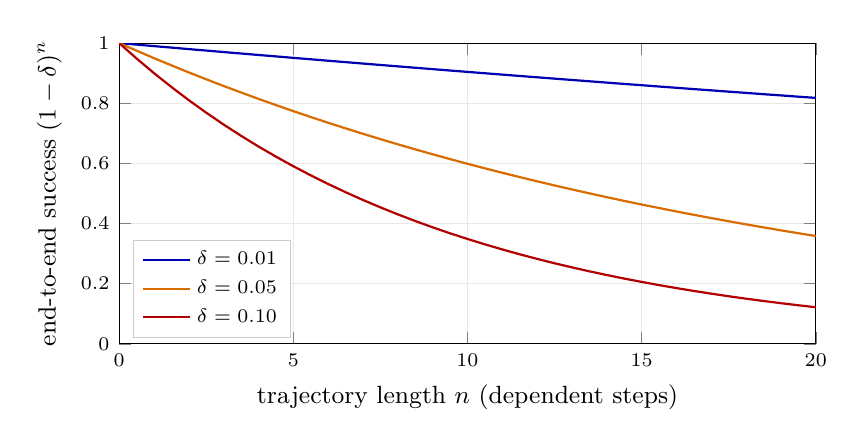
\begin{tikzpicture}
\begin{axis}[
  width=0.86\linewidth, height=5.4cm,
  xlabel={trajectory length $n$ (dependent steps)},
  ylabel={end-to-end success $(1-\delta)^n$},
  xmin=0, xmax=20, ymin=0, ymax=1,
  xtick={0,5,10,15,20}, grid=both, grid style={gray!18},
  legend cell align=left,
  legend style={font=\scriptsize, at={(0.02,0.02)}, anchor=south west, draw=gray!40},
  tick label style={font=\scriptsize}, label style={font=\small},
]
\addplot[thick, blue!70!black, domain=0:20, samples=41] {0.99^x};
\addplot[thick, orange!85!black, domain=0:20, samples=41] {0.95^x};
\addplot[thick, red!70!black, domain=0:20, samples=41] {0.90^x};
\legend{$\delta=0.01$, $\delta=0.05$, $\delta=0.10$}
\end{axis}
\end{tikzpicture}
\caption{The trajectory inversion. When success requires $n$ dependent steps to
all hold, end-to-end success is $(1-\delta)^n$, where the per-step failure rate
$\delta$ is the single-turn residual $R$ of Section~\ref{sec:arch}. The layers of
this paper lower $\delta$ (shift between curves) but cannot change $n$ (position
along a curve); at $\delta=0.05$, ten steps already cost $40\%$ of successes.}
\label{fig:agentic}
\end{figure}

\textbf{Failures are correlated ($\rho_c > 1$).} The multiplicative-decay argument
is exact only when $\rho_c = 1$, and the real world violates this: a hard input
can defeat several layers at once. Measuring $\rho_c$ empirically, and designing
layers to be maximally decorrelated so that $\rho_c$ stays near $1$, is an open and
practically urgent problem, and the term that a naive component-by-component
optimization silently sets to $1$.

\textbf{There is no end-to-end reliability budget.} The field optimizes
components (a better retriever, a better judge) without a shared framework for
allocating a fixed error/latency/cost budget across the whole pipeline. The
reference architecture above is a sketch of what such a framework would
instrument, not a solution.

\section{Conclusion}

Reliable LLM applications are not built by discovering one decisive technique;
they are engineered by composing many imperfect ones. We organized the field's
sprawling toolbox into four composable layers, evaluation, retrieval quality,
inference-time reliability, and guardrails, mapped common failures to the layer
that most cheaply catches them, and argued that reliability emerges from
defense in depth: cheap filters, ordered by cost, where distinct filters extend
coverage across failure classes and redundant, independent filters drive the
residual of a shared class down multiplicatively. The framing turns a
reading list into an architecture and exposes the discipline's real frontier,
not any single missing method, but trustworthy evaluation, calibrated
abstention, reliability that survives lengthening agent trajectories, and a
principled way to spend a fixed reliability budget across the whole stack.

{\small
\bibliographystyle{plainnat}
\bibliography{refs}
}

\end{document}
